\documentclass[10pt]{beamer}

% Theme Selection
\usetheme{Madrid}
\usecolortheme{default}

\usepackage[style=apa,backend=biber]{biblatex}
\addbibresource{refs.bib}

% Packages for Diagrams
\usepackage{tikz}
\usepackage{tikz-cd}
\usetikzlibrary{positioning, arrows.meta, shapes, calc, fit}
\usepackage{graphicx}
\usepackage{amsthm}

% Metadata
\title[The Categorical Cerebellum]{Categorical Cerebellum}
\subtitle{Ideas to propose an unified cerebellar computation}
\author{Luis Luarte}
\date{\today}

\begin{document}
	
	% --- SLIDE 1: Title ---
	\begin{frame}
		\titlepage
	\end{frame}
	
	% --- SLIDE 2: The Computational Unit ---
	\begin{frame}{1. Computational unit: the microzone}
		The fundamental operational unit of the cerebellum is the \textbf{Corticonuclear Microcomplex} (Microzone).
		
		\begin{columns}
			\column{0.5\textwidth}
			\textbf{Anatomy \& Connectivity:}
			\begin{itemize}
				\item \textbf{Input 1 (Context):} Mossy Fibers $\to$ Granule Cells ($\sim$50 billion) $\to$ Parallel Fibers. \textit{Expands state space.}
				\item \textbf{Input 2 (Error):} Climbing Fibers (from Inferior Olive). \textit{1-to-1 mapping with Purkinje Cells.}
				\item \textbf{Output:} Purkinje Cells (GABAergic/Inhibitory) $\to$ Deep Cerebellar Nuclei (DCN).
			\end{itemize}
			
			\column{0.5\textwidth}
			\centering
			% TikZ Diagram of Microcircuit
			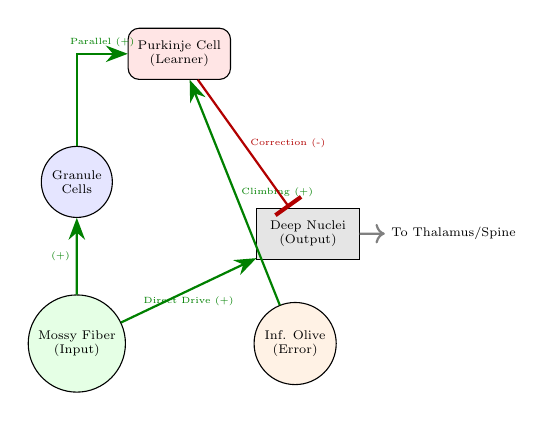
\begin{tikzpicture}[
				scale=0.65, transform shape,
				node distance=1.5cm,
				% Define Node Styles
				neuron/.style={draw, circle, minimum size=1cm, align=center, font=\scriptsize},
				purkinje/.style={neuron, rectangle, rounded corners, fill=red!10, minimum width=2cm},
				granule/.style={neuron, fill=blue!10},
				mossy/.style={neuron, fill=green!10},
				dcn/.style={neuron, rectangle, fill=gray!20, minimum width=2cm},
				olive/.style={neuron, fill=orange!10},
				% Define Canonical Arrow Styles
				excitatory/.style={->, -{Stealth[scale=1.2]}, thick, green!50!black},
				inhibitory/.style={->, -{Bar[width=4mm, line width=1.5pt]}, thick, red!70!black}
				]
				% Nodes
				\node[purkinje] (PC) {Purkinje Cell\\(Learner)};
				\node[granule, below left=1.5cm and 0.5cm of PC] (GC) {Granule\\Cells};
				\node[dcn, below right=2.5cm and 0.5cm of PC] (DCN) {Deep Nuclei\\(Output)};
				\node[mossy, below=1.5cm of GC] (MF) {Mossy Fiber\\(Input)};
				\node[olive, right=2.5cm of MF] (IO) {Inf. Olive\\(Error)};
				
				% Excitatory Connections (Green / Arrowhead)
				\draw[excitatory] (MF) -- (GC) node[midway, left, font=\tiny] {(+)};
				\draw[excitatory] (GC) |- (PC) node[near end, above, font=\tiny] {Parallel (+)};
				\draw[excitatory] (MF) -- (DCN) node[midway, below, font=\tiny] {Direct Drive (+)};
				\draw[excitatory] (IO) -- (PC) node[midway, right, font=\tiny] {Climbing (+)};
				
				% Inhibitory Connections (Red / T-Bar)
				\draw[inhibitory] (PC) -- (DCN) node[midway, right, font=\tiny] {Correction (-)};
				
				% Output Arrow
				\draw[->, thick, gray] (DCN) -- +(1.5,0) node[right, black, font=\scriptsize] {To Thalamus/Spine};
				
			\end{tikzpicture}
		\end{columns}
		
		\vspace{0.5cm}
		\textbf{Mechanism:} The Purkinje cell learns to predict and cancel sensory discrepancies via \textbf{LTD} (Long-Term Depression) at the Parallel Fiber synapse, gated by the Climbing Fiber error signal.
	\end{frame}
	
	% --- SLIDE 3: Structural Homogeneity ---
	\begin{frame}{2. Anatomical homogeneity}
		\begin{itemize}
			\item Regular structure \parencite{ecclesCerebellumNeuronalMachine1967}
			\item Structure based inference lead to `dysmetria of thought' \parencite{schmahmannDysmetriaThoughtClinical1998}
			\item `Consensus' paper of cerebellum role in motor and cognition control \parencite{koziolConsensusPaperCerebellums2014}
			\item This ultimately lead to the universal cerebellar transform \parencite{itoCerebellarCircuitryNeuronal2006,schmahmannMovementThoughtAnatomic1996}
		\end{itemize}
	\end{frame}
	
	\begin{frame}{3. The hypothesis: the universal cerebellar transform}
		\begin{figure}[h!]
			\centering
			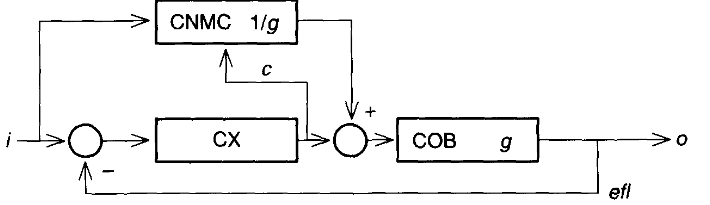
\includegraphics[width=0.75\linewidth]{p1.png}
			\label{fig:ito_model}
		\end{figure}
		
		\begin{itemize}
			\item $i$ move the hand 10 cm.
			\item physics $g$ offers $80\%$ resistance, so $i \cdot g = 8 cm.$
			\item cerebellum get a copy of $i$ from CX and learns the inverse function
			\item Amplify hand force by $1.25$ as $1/0.8 = 1.25$
			\item CNMC generates motor command $i \cdot (1/g)$ (e.g. push 1.25 harder)
			\item $\text{Outcome} = (i \cdot \frac{1}{g}) \cdot g = i$
		\end{itemize}
	\end{frame}
	
	\begin{frame}{4. The challenges to Ito's control theory}
		\begin{figure}
			\centering
			
\includegraphics[width=0.55\linewidth]{p2.png}
			\caption{\parencite{pasalarForceFieldEffects2006}}
		\end{figure}
		
		\begin{itemize}
			\item Intercept and track task with viscosity (force) and elasticity (position)
			\item $f(\theta) = \beta_{0} + \beta_{1} \cdot exp(k_{1} \cdot cos(\theta - \mu_{1})) +
			\beta_{2} \cdot exp(k_{2} \cdot cos(\theta - \mu_{2}))$
			\item $\theta : \text{position along the circle}$, $\mu : \text{P-cells preferred direction in circle}$
			\item $k : \text{width of tunning curves, inverse of sd}$
		\end{itemize}
	\end{frame}
	
	\begin{frame}{4. The challenges to Ito's control theory}
		\begin{figure}
			\centering
			
\includegraphics[width=0.55\linewidth]{p3.png}
		\end{figure}
		\begin{itemize}
		\item No force model $f(\theta) = \beta_{0} + \beta_{1} \cdot exp(k_{1} \cdot cos(\theta - \mu_{1})) \dots$
		\item Force model $f(\theta) = \beta_{0} + \beta_{1} \cdot F + (\beta_{2} + \beta_{3}F) \cdot exp(k_{1} \cdot cos(\theta - \mu_{1})) \dots$
		\item P-cells encoding state space $\theta$ with $R^{2} > 0.5$
		\item Adding `forces' does not improve the model, thus cerebellum does not output $1/g$
		\end{itemize}
	\end{frame}
	
	\begin{frame}{4. The challenges to Ito's control theory}
	\begin{figure}
		\centering
		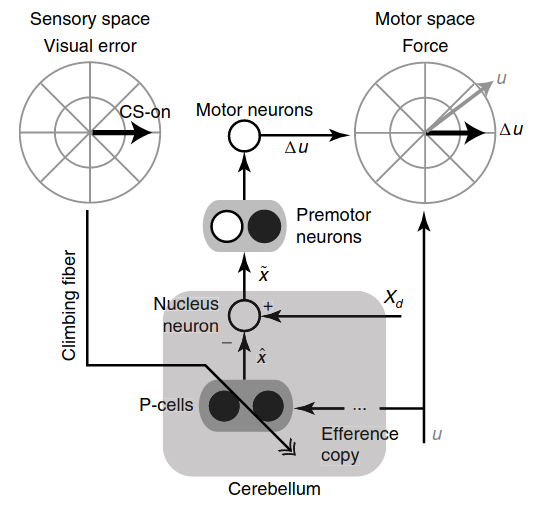
\includegraphics[width=0.45\linewidth]{p5.png}
	\end{figure}
	\begin{itemize}
		\item $\text{Climbing fiber} \xrightarrow{Glutamate} \text{P-cell} \rightarrow \text{Complex Spike} \xrightarrow{DAG_{\text{parallel fibers}} + PKC} \text{LTD} \rightarrow \text{SS}$
		\item CS encode the tuple ($Space_{tuning}, Magnitude_{timing}$)
		\item $\hat{x}$ is the predicted state (inhibitory) and merges with $X_{d_{\text{mossy fibers}}}$ at deep nuclei to form $\widetilde{x}$ correction signal
	\end{itemize}
\end{frame}

\begin{frame}{4. The challenges to Ito's control theory}
	\begin{itemize}
		\item \cite{itoMovementThoughtIdentical1993} model is a inverse dynamics controller, however, P-cells do not encode `required forces'
		\item \cite{herzfeldEncodingErrorLearning2018} shows that P-cells are forward models enconding the sensory consequences of the movement
		\item Climbing fibers goes from simple binary signal to a complex signal tuple (Spatial, Magnitude)
		\end{itemize}
\end{frame}

\begin{frame}{5. The nail in the coffin (?)}
	\begin{figure}
		\centering
		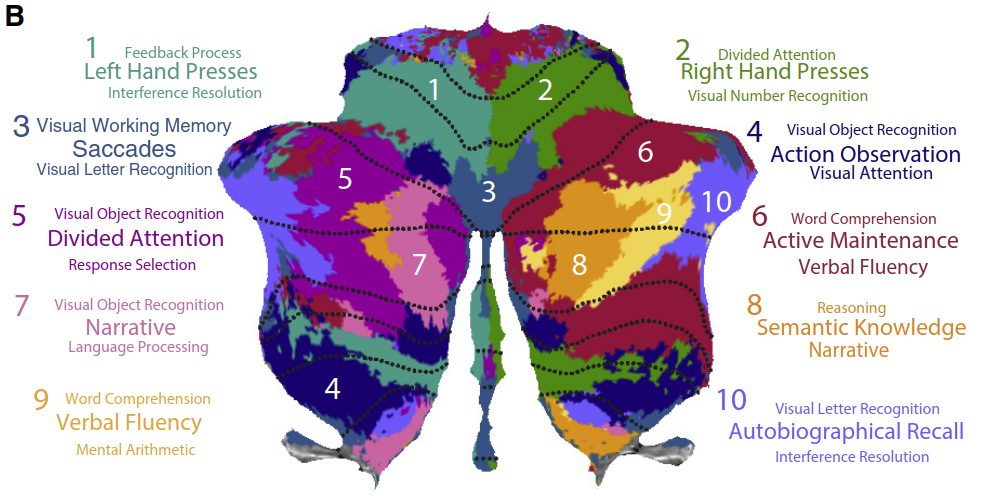
\includegraphics[width=0.8\linewidth]{p6.png}
		\caption{\cite{diedrichsenUniversalTransformMultiple2019}}
	\end{figure}
	\begin{itemize}
		\item Some parcellations do not follow anatomical lobules
		\item Parcellations seems to be highly specialized
	\end{itemize}
\end{frame}

\begin{frame}{6. My rebuttal to King, Diedrichsen and others}
	\begin{itemize}
		\item The `projector' trap: cortex projects color lights onto a white screen (cerebellum)
		\item Mistake the input partition (projection) for white screen functionality
		\item If you feed motor data $(A)$ into the machine you get motor correction $(A')$
		\item If you feed social data $(B)$ into the machine you get social correction $(B')$
		\item \cite{diedrichsenUniversalTransformMultiple2019} sees $A \neq B$ and concludes that the machine has changed
		\item What's missing: the transformation $T$ could be identical $T(A) \cong T(B)$
	\end{itemize}
	
	\begin{equation*}
		\begin{tikzcd}[row sep=huge, column sep=huge, ampersand replacement=\&]
			% Nodes
			\text{Cortical Input } (X_d) 
			\arrow[r, "\text{Granule Expansion}"] 
			\arrow[d, "\text{Excitatory Drive (+)}"', bend right=45] 
			\& 
			\text{Basis Function } (\Phi(X)) 
			\arrow[d, "\text{Purkinje Weights } (w)"] 
			\\
			\text{Correction Output } (\Delta u) 
			\& 
			\text{State Prediction } (\hat{x}) 
			\arrow[l, "\text{Nucleus Inhibition (-)}"]
		\end{tikzcd}
	\end{equation*}
	
\end{frame}

\begin{frame}{7. Granule expansion permits a universal construct}
	$\Phi : (\mathcal{M} \cup \mathcal{S}) \rightarrow \mathcal{H}$, granule cell expasion lifts a into an enormous state space from mossy fibers $\mathbb{R}^{N}$ into $\mathbb{R}^{1000N}$, as each granule cell receives synaptic input from 3-4 mossy fibers.
	\begin{itemize}
		\item \cite{huangConvergencePontineProprioceptive2013} showed structural multimodal input convergence into granule cells
		\item \cite{ishikawaMultimodalSensoryIntegration2015} showed functional multimodal input convergence into granule cells
		\item $\Phi : \mathcal{M} \times \mathcal{S} \rightarrow \mathcal{H}$, can be supported as granule cell expansion is extremelly sparse, few connections active at a time
		\item We get from \cite{herzfeldEncodingErrorLearning2018} modification of UCT $\Delta w = - \eta \cdot \underbrace{\text{Duration}(CF)}_{\text{Magnitude } \alpha} \cdot \underbrace{1_{CF}}_{\text{Direction } \vec{e}} \cdot \underbrace{\Phi(u)}_{\text{Context}}$
	\end{itemize}
\end{frame}

\begin{frame}{Disclaimer}
	Just learning category theory.
\end{frame}

\begin{frame}{1. The Category and axioms}
	\begin{block}{Definition: The Category ($\mathcal{C}$)}
		A category consists of:
		\begin{itemize}
			\item \textbf{Objects:} A collection $Ob(\mathcal{C})$ (e.g., $A, B, C$).
			\item \textbf{Morphisms:} Arrows between objects, $f: A \to B$.
			\item \textbf{Composition:} An operation $\circ$ linking arrows path-wise.
		\end{itemize}
	\end{block}
	
	\begin{block}{Axioms}
		\begin{enumerate}
			\item \textbf{Associativity:} The sequence matters, not the grouping.
			\[ (h \circ g) \circ f = h \circ (g \circ f) \]
			\item \textbf{Identity:} Every object has a "Do Nothing" arrow ($id_A$).
			\[ f \circ id_A = f \quad \text{and} \quad id_B \circ f = f \]
		\end{enumerate}
	\end{block}
\end{frame}

\begin{frame}{1. The Category and axioms}
	\begin{figure}
		\centering
		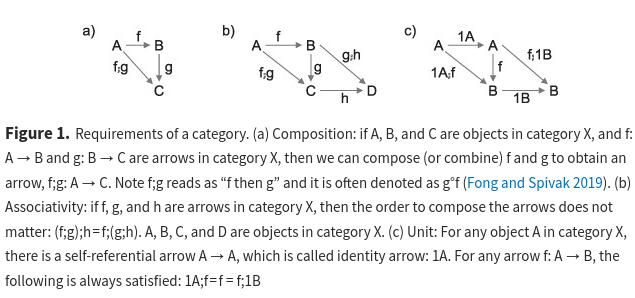
\includegraphics[width=0.9\linewidth]{p7.png}
		\caption{\cite{tsuchiyaRelationalApproachConsciousness2021}}
	\end{figure}

\end{frame}

% SLIDE 2: Structure and Translation
\begin{frame}{2. Isomorphism and Functors}
	\begin{block}{Isomorphism (Structural Equality)}
		Two objects $A$ and $B$ are isomorphic ($A \cong B$) if there exist inverses:
		\[ g \circ f = id_A \quad \text{and} \quad f \circ g = id_B \]
		Structurally the same; information is preserved perfectly during conversion.
	\end{block}
	
	\vspace{0.5cm}
	
	\begin{block}{Functor (The Map Between Categories)}
		A mapping $F: \mathcal{C} \to \mathcal{D}$ that preserves structure:
		\begin{itemize}
			\item Maps objects to objects: $F(A) \in \mathcal{D}$
			\item Maps arrows to arrows: $F(f): F(A) \to F(B)$
			\item Preserves composition: $F(g \circ f) = F(g) \circ F(f)$
		\end{itemize}
		A "Translation" or "Model" that keeps connections intact.
	\end{block}
\end{frame}

\begin{frame}{The Endofunctor: Modeling System Change}

	\begin{block}{Definition}
		An \textbf{endofunctor} is a functor that maps a category to itself:
		\[ F: \mathcal{C} \longrightarrow \mathcal{C} \]
		It takes every object and morphism in $\mathcal{C}$ and maps them to objects and morphisms within the \textbf{same} category.
	\end{block}
	
	\vspace{0.3cm}
	
	\begin{block}{Intuition: The "System Update"}
		
		$F$ as a time-step operator ($t \to t+1$).
		\begin{itemize}
			\item The "Hardware" (Objects like Neuronal Populations) remains constant.
			\item The "Software" (Morphisms like Synaptic Weights) are updated.
		\end{itemize}
	\end{block}
\end{frame}

% --- SLIDE 2: The Biological Mechanism ---
\begin{frame}{The Endofunctor in the Cerebellum}
	\begin{center}
		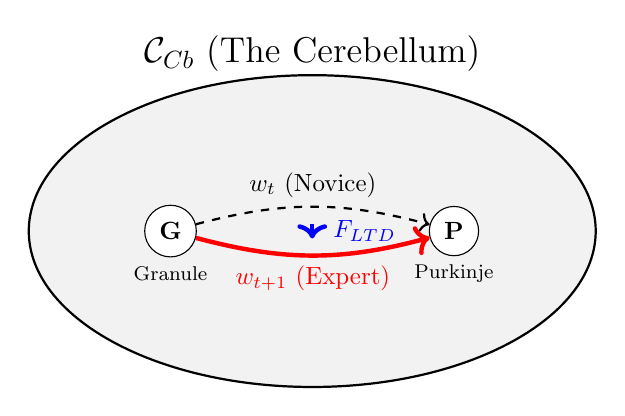
\begin{tikzpicture}[scale=0.9, every node/.style={scale=0.9}]
			% Draw the category bubble
			\draw[thick, fill=gray!10] (0,0) ellipse (4cm and 2.2cm);
			\node at (0, 2.5) {\Large $\mathcal{C}_{Cb}$ (The Cerebellum)};
			
			% Nodes inside (Hardware)
			\node (G) at (-2, 0) [circle, draw, fill=white] {\textbf{G}};
			\node (P) at (2, 0) [circle, draw, fill=white] {\textbf{P}};
			\node at (-2, -0.6) {\footnotesize Granule};
			\node at (2, -0.6) {\footnotesize Purkinje};
			
			% Morphism at time t (Novice)
			\draw[->, thick, dashed] (G) to [bend left=15] node[above] {$w_t$ (Novice)} (P);
			
			% Morphism at time t+1 (Expert)
			\draw[->, ultra thick, red] (G) to [bend right=15] node[below] {$w_{t+1}$ (Expert)} (P);
			
			% The Endofunctor Arrow indicating the change
			\draw[->, blue, ultra thick, shorten >=5pt, shorten <=5pt] (0, 0.3) -- (0, -0.3);
			\node at (0, 0) [right, xshift=5pt, blue] {$F_{LTD}$};
		\end{tikzpicture}
	\end{center}
	
	\vspace{0.2cm}
	
	\begin{block}{The Biological Endofunctor}
		In the cerebellum, the anatomy ($G, P$) does not change during learning. Only the function ($w$) changes.
		
		Therefore, the \textbf{Climbing Fiber Learning Rule (LTD)} is physically an Endofunctor acting on the category $\mathcal{C}_{Cb}$.
	\end{block}
\end{frame}

\begin{frame}{1. Defining the Neuro-Category $\mathcal{C}_{Cb}$}
	We construct a category where neuronal populations are objects and fiber connections are morphisms.
	
	\begin{block}{The Objects (Vector State Spaces)}
		Distinct nuclei define the processing stages:
		\begin{itemize}
			\item \textbf{$M$ (Mossy Fibers):} Input Context space ($\mathbb{R}^{in}$).
			\item \textbf{$G$ (Granule Cells):} High-Dim Basis space ($\mathbb{R}^{sparse}$).
			\item \textbf{$P$ (Purkinje Cells):} Prediction space ($\mathbb{R}^{out}$).
			\item \textbf{$D$ (Deep Nuclei):} Actuator/Comparator space.
		\end{itemize}
	\end{block}
	
	\begin{block}{The Morphisms (Synaptic Transfer Functions)}
		Anatomical connections define the computational arrows:
		\begin{itemize}
			\item \textbf{$\Phi: M \to G$ (Expansion):} Non-linear basis projection.
			\item \textbf{$w: G \to P$ (Weights):} Linear sum via Parallel Fibers.
			\item \textbf{$-: P \to D$ (Inhibition):} Sign inversion to Deep Nuclei.
			\item \textbf{$Id: M \to D$ (Drive):} Direct excitatory collaterals.
		\end{itemize}
	\end{block}
\end{frame}

% --- SLIDE 2: The Diagram ---
\begin{frame}{2. Resulting diagram}
	\begin{center}
		% Adjusting row and column separation for clarity
\begin{tikzcd}[row sep=2cm, column sep=2.5cm, ampersand replacement=\&]
	% --- Row 1 ---
	% Node 1-1: Mossy Fibers
	M \text{ (Mossy Input)}
	\arrow[r, "\Phi \text{ (Expand)}"]
	% Drive arrow: Needs to go to D (Row 3, Col 2)
	% 'rdd' = Right 1, Down 2
	\arrow[rdd, "Id \text{ (Drive +)}"', near start, bend right=20, very thick]
	\&
	% Node 1-2: Granule Cells
	G \text{ (Granule Basis)}
	\arrow[d, "w_{PF} \text{ (Learn)}"]
	\\
	% --- Row 2 ---
	% Node 2-1: Inferior Olive (Added to fix the error)
	IO \text{ (Olive Error)}
	% Teacher Arrow: From IO to P
	\arrow[r, dashed, "\text{Teacher (LTD)}", blue]
	\&
	% Node 2-2: Purkinje Cells
	P \text{ (Purkinje Predict)}
	\arrow[d, "- \text{ (Inhibit)}", very thick]
	\\
	% --- Row 3 ---
	\&
	% Node 3-2: Deep Nuclei
	D \text{ (Deep Nuclei Output)}
\end{tikzcd}
	\end{center}
\end{frame}

% --- SLIDE 3: The Axiomatic Derivations ---
\begin{frame}{3. Biological Emergence from Axioms}
	By forcing the anatomy to obey categorical axioms, specific biological functions emerge necessarily.

	\begin{columns}
		% LEFT COLUMN: Composition
		\begin{column}{0.48\textwidth}
			\begin{block}{Axiom: Composition ($h \circ g \circ f$)}
				The existence of the path $M \to G \to P \to D$ implies a composite arrow exists.
				\[ \text{Composite} = (-) \circ w_{PF} \circ \Phi \]
			\end{block}
			\textbf{Biological Emergence: Internal Simulation}
			The brain possesses a direct transformation from Input ($M$) to Predicted Outcome ($D$) without requiring physical movement. This is the definition of a \textbf{Forward Model}.
		\end{column}
		
		% RIGHT COLUMN: Commutativity
		\begin{column}{0.48\textwidth}
			\begin{block}{Axiom: Commutativity}
				The Deep Nuclei ($D$) integrate two converging paths. The diagram must resolve consistently.
				\[ \text{Output}_D = \text{Path}_1 + \text{Path}_2 \]
			\end{block}
			\textbf{Biological Emergence: Subtraction}
			Combining the Drive (+) and Inhibition (-) paths:
			\[ D = \text{Drive}(M) - \text{Prediction}(P) \]
			The DCN is physically forced to act as a \textbf{Comparator}, outputting only the corrective error vector ($\Delta u$).
		\end{column}
	\end{columns}
\end{frame}

\begin{frame}{3. Biological Emergence from Axioms}
	How do we model learning in Category Theory?
	
	The Climbing Fiber is not just an input data source; it is an operator that transforms the system's internal functions.
	
	\vspace{0.5cm}
	
	\begin{block}{The Axiom: The Endofunctor}
		Learning is a map from the category at time $t$ to time $t+1$. 
		The error signal induces a \textbf{Functorial Update} ($F_{error}$) that modifies the morphism $w$ (weights) while preserving the objects ($G$ and $P$).
	\end{block}
	
	\vspace{0.3cm}
	
	\begin{block}{The "Arrow of Arrows"}
		Mathematically, we are mapping one function to another:
		\[ F_{error}: (w: G \to P) \longmapsto (w': G \to P) \]
		This implies the cerebellum is not just computing a state; it is constantly \textbf{computing its own structure}.
	\end{block}
\end{frame}

% --- SLIDE 2: The Mechanism & Diagram ---
\begin{frame}{3. Biological Emergence from Axioms}
	\begin{block}{Biological Emergence: Structural Plasticity}
		This mathematical update is physically implemented by Long-Term Depression (LTD). The error signal (Calcium spike) depresses specific synapses, effectively "bending" the function.
	\end{block}
	
	\vspace{0.5cm}
	
	\begin{center}
		\textbf{Visualizing the Weight Transformation}
		% The diagram shows the transition from old weight to new weight caused by the error
		\begin{tikzcd}[row sep=huge, column sep=huge, ampersand replacement=\&]
			G \text{ (Granule Basis)}
			% The "Old" weight arrow (bottom)
			\arrow[r, "w_{t} \text{ (Novice)}"', ""{name=A, above}]
			% The "New" weight arrow (top, bent)
			\arrow[r, bend left=50, "w_{t+1} \text{ (Expert)}", ""{name=B, below}]
			\&
			P \text{ (Purkinje Predict)}
			% The Error arrow acting ON the weight arrows
			\arrow[from=A, to=B, dashed, blue, thick, "\text{CF Error (LTD)}", shorten >=5pt, shorten <=5pt]
		\end{tikzcd}
	\end{center}
\end{frame}

\begin{frame}{How does the method continues}
	\begin{itemize}
		\item Traced categories to define the `loop' brain-cerebellum back to brain
		\item The `learner' category where the computational model is specified
		\item Functors between all categories allows us to specify our models in context, and avoid ad-hoc specifications
	\end{itemize}
\end{frame}

\begin{frame}{Experimental output}
	\begin{itemize}
		\item Passing all axioms guarantees that specification can be turned into a single composed and unified function
		\item The composition is a computational model that can be tested with usual methodologies
		\item Furthermore, categorical specification under composition allows to generate precise hypothesis
		\item We can test pertubation of `computations' and track them to biological strucure
		\item Or propose a biological perturbation and determine affected computations
	\end{itemize}
\end{frame}


	
\end{document}